% !TeX encoding = windows-1251
\documentclass[fullscreen=true,russian,compress,%
	hyperref={unicode,bookmarks=false}]{presentation}
\inputencoding{utf8} % Кодировка вашего файла
% Внимание! Опция russian не совместима с \tableofcontents
\usepackage[russian]{babel} % Эту строку можно удалить
\usepackage{paratype} % Выбираем шрифт
% Определяем длины частей нижнего колонтитула: автор, название, число слайдов
\makefootline{.35}{.55}{.1} % Сумма длин = 1

\usepackage{tikz} % Для создания рисунков с помощью tikz
\usepackage{listings} % Для листингов программ

\begin{document}

% Если потребуется, переводим названия блоков с английского:
\deftranslation[to=Russian]{Theorem}{Теорема}
\deftranslation[to=Russian]{Example}{Пример}

% Данные титульного слайда
\title[Презентация в \texttt{beamer}]{Делаем презентацию в \texttt{beamer}}
\author{Александр Александрович Александров}
\institute{Научный руководитель: Р.\,Р.~Разумный}
\date{17.06.2017}

% Создаем титульный слайд
\begin{frame}
\titlepage
\end{frame}

% \tableofcontents не работает при включенной опции russian пакета babel
%\begin{frame}{Содержание}\tableofcontents\end{frame}

\section{Вступление}

\begin{frame}{Вступление}

\begin{block}{Подробное описание пакета \texttt{beamer}}
T.~Tantau, J.~Wright, V.~Mileti\'c,
\href{https://www.ctan.org/tex-archive/macros/latex/contrib/beamer}{The beamer class}, занимает \textbf{248 с.}
\end{block}	

\begin{block}<2->{Цель презентации}
	Упростить подготовку презентации для выпускников ф-та ИВТ ЯрГУ.
\end{block}	

\visible<3->{
\begin{block}{Задачи:}
	\begin{enumerate}
	\item<3-> Сформулировать основные правила подготовки презентации.
	\item<4-> Ознакомиться с возможностями пакета \texttt{beamer}.
	\item<5-> Подготовить стилевой файл и пример презентации.
	\end{enumerate}
\end{block}	
}
\end{frame}


\section{Правила подготовки презентации}

\begin{frame}{С чего начать}
\begin{block}{Подготовка}
	\begin{enumerate}
		\item Выпишите все основные моменты, о которых вы хотите сказать.
		\item Разбейте на 2--3 раздела.
		\item Не забывайте про <<Правило неосведомленности аудитории>>.
	\end{enumerate}
\end{block}

\begin{block}{Длительность и объем}
	\begin{enumerate}
		\item Выясните, сколько времени отводится ваш доклад.
		\item Презентация одного слайда занимает (в среднем) 1-2 минуты.
		\item Обычный слайд содержит 20--40 слов (максимум 80).\\ 
		Пример: на этом слайде 50 слов.
		\item Используйте иллюстрации, \\
		о~деталях сообщайте в устном докладе \\
		или выносите их в приложение. \ 
		\label{labstr}\hyperlink{example}{\beamerbutton{Пример}}
		%\item Всё, что не укладывается в эти рамки, вынесите в приложения.
	\end{enumerate}
\end{block}

\end{frame}

\begin{frame}{Советы по оформлению слайда}
	\begin{enumerate}
		\item Название каждого слайда должно быть информативным.
		\item Структурируйте текст \textbf{по смыслу}\\ 
		с помощью списков, блоков и колонок.    
		\item Используйте \textbf{\textbackslash{}textbf} и \alert{\textbackslash{}alert}
		для выделения важного.\\
		\textbf{Но не чрезмерно!}
		\item Короткие фразы лучше, чем предложения.\\
		(После фраз точки не ставятся.)
		\item Разделяйте строки вручную по смыслу (с помощью \textbackslash\textbackslash).  
		\item Шрифт --- sans serif (без засечек).
		\item Избегайте нумерации теорем и формул.\\
		Вместо этого придумайте метки или названия.
		\item Размер символов на рисунке такой же, как и в тексте.
		%\item По возможности, вместо формул ипользуйте текст.	
	\end{enumerate}
\end{frame}

\begin{frame}{Пример структурированного текста}
	\begin{columns}[T]
		\begin{column}{.35\paperwidth}
			\framezoom<1><2>[border](2.0cm,1.4cm)(1.5cm,1.0cm) % Для зуммирования
			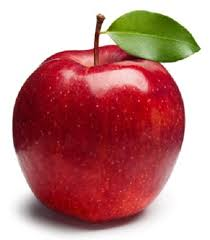
\includegraphics[width=\textwidth]{apple.jpg} 
		\end{column}
		\begin{column}{.5\paperwidth}
			\begin{theorem}[Ньютон, 1699]
				\centering
				\(\int\limits_a^b f(x)\,dx = \Phi(a) - \Phi(b)\)
			\end{theorem}
			\begin{proof}
				Поля слишком малы.
			\end{proof}
			\begin{example}
				\centering
				\(\int\limits_0^{\pi} \sin x\,dx = - \cos \pi - (- \cos 0) = 2\)
			\end{example}
		\end{column}
	\end{columns}
\end{frame}

% Настраиваем стиль листинга
\lstset{%
	language=[LaTeX]TeX,
	showstringspaces=false,
	basicstyle=\footnotesize\ttfamily\color{blue!35!black},
	keywordstyle=\bfseries\color{blue!80!black},
	%commentstyle=\it\color{black!60},
	identifierstyle=\color{black},
	%stringstyle=\color{black!60},
	%deletetexcs={fill},  
	emph={\filldraw, \node},
	emphstyle={\color{red!80!black}},
	emph={[2]circle},          % emphasized words 2
	emphstyle={[2]\color{blue!50!green}}, 	
	morecomment=[s][\color{black!60}]{[}{]},
	tabsize=2
}

% Не забывайте добавлять опцию [fragile] к тем слайдам,
% где приводятся листинги программ
\begin{frame}[fragile]{Пример листинга программы}
	\begin{columns}[T]
		\begin{column}{.6\paperwidth}
			\begin{block}{Исходный код}
				\begin{lstlisting}
\begin{tikzpicture}[scale=0.5]
  \filldraw[fill=green, fill opacity=0.4] 
      (0,-1) circle (2);
  \filldraw[fill=blue, fill opacity=0.4] 
      (0,1) circle (2);
  \node at (0,2) {NP};
  \node at (0,0) {P};
  \node at (0,-2) {co-NP};
\end{tikzpicture}
				\end{lstlisting}
			\end{block}
		\end{column}
		\begin{column}{.15\paperwidth}
			\begin{block}{Результат}
				%		\begin{center}
				\ \\
				\centering	
				\begin{tikzpicture}[scale=0.5]
				\filldraw[fill=green, fill opacity=0.4] (0,-1) circle (2);
				\filldraw[fill=blue, fill opacity=0.4] (0,1) circle (2);
				\node at (0,2) {NP};
				\node at (0,0) {P};
				\node at (0,-2) {co-NP};
				\end{tikzpicture}
				%		\end{center}
			\end{block}
		\end{column}
	\end{columns}
\end{frame}

\section{Заключение}

\begin{frame}{Заключение}
	\begin{center}
	\LARGE 
	Подводим итоги.\\
	Описываем перспективы.
	\end{center}
\end{frame}

\begin{frame}%[allowframebreaks]
	\frametitle<presentation>{Литература}
	
	\begin{thebibliography}{9}
		\beamertemplatebookbibitems
		
		\bibitem{Baldin:2013}
		Е.\,М.~Балдин.
		\newblock {\em \href{https://www.ctan.org/tex-archive/info/russian/Computer_Typesetting_Using_LaTeX}{Компьютерная типография \LaTeX.}}
		\bibitem{Beamer:2017}
		Till Tantau, Joseph Wright, Vedran Mileti\'c.
		\newblock {\em \href{https://www.ctan.org/tex-archive/macros/latex/contrib/beamer}{The beamer class.}}
		\bibitem{BeamerThemes}
		{\em\href{https://www.hartwork.org/beamer-theme-matrix/}{Таблица стилей}}
		
	\end{thebibliography}
\end{frame}

\appendix


\begin{frame}{Основные части презентации}
	\label{example}
	\begin{description}
		\item[Вступление:] о чем пойдет речь.
		\item[Основная часть:] что удалось выяснить, обнаружить.
		\item[Заключение:] повторяем основную мысль.\\
		(После этого можно описать перспективы.) 
		\item[Литература:] не более одного слайда.\\
		Только действительно полезные ссылки.
		\item[Приложение:] все, что не поместилось в основной части,\\
		а также ответы на ожидаемые вопросы.
	\end{description}
	\centering
	\hyperlink{labstr}{\beamerbutton{Назад}}
\end{frame}

\begin{frame}{Пример оверлеев в beamer}
	\begin{block}{Оверлеи}
		2. \only<2->{Со второго} слайда\\
		\visible<3->{3. С третьего\\}
		\uncover<4->{4. С четвертого\\}
		\visible<1,3,5>{5. Мелькает\\}
		6. \alt<4->{Больше трех}{Меньше четырех} \\
		7. \temporal<3,4>%
		{\color{red}}{\color{yellow}}{\color{green}}%	
		Меняет цвет
	\end{block}
\end{frame}


\end{document}

